\documentclass[a0,portrait]{a0poster}


\usepackage{multicol}
\columnsep=100pt
\columnseprule=3pt

\usepackage[svgnames]{xcolor}

\usepackage{palatino}

\usepackage[]{sourcecodepro}

\usepackage{graphicx}
\graphicspath{{figs/}}
\usepackage{booktabs}
\usepackage[font=small,labelfont=bf]{caption}
\usepackage{amsfonts, amsmath, amsthm, amssymb}
\usepackage{wrapfig}

\usepackage{nicefrac}
\usepackage{bm}
\usepackage{siunitx}
\usepackage{tikz}
\usepackage{pgfplots}
\usetikzlibrary{positioning}
\usetikzlibrary{arrows.meta}
\usepgfplotslibrary{groupplots}

\definecolor{darkblue}{HTML}{00688B}
\definecolor{darkgreen}{HTML}{6E8B3D}
\definecolor{cadet}{HTML}{DAE1FF}
\definecolor{salmon}{HTML}{FFB08A}

\begin{document}

\begin{minipage}[b]{1.0\linewidth}
  \veryHuge \color{NavyBlue}
  \textbf{
    \noindent A step towards reduced order modelling of flow characterized \\
    by wakes using Proper Orthgonal Decomposition
  }
  \color{Black}\\
\end{minipage}
\begin{minipage}[b]{0.7\linewidth}
  \huge \textbf{Eivind Fonn, Mandar Tabib, Adil Rasheed, Trond Kvamsdal}\\[0.5cm]
  \huge SINTEF Digital\\[0.4cm]
  \Large \texttt{eivind.fonn@sintef.no} --- +47 41 44 98 89\\
\end{minipage}
%
\begin{minipage}[b]{0.25\linewidth}
  \includegraphics[width=20cm]{common/sintef}\\
\end{minipage}

\vspace{1cm}

\begin{multicols}{2}

\color{DarkSlateGray}
\Large

\section*{\LARGE Introduction}

\textbf{Problem:} High fidelity simulations of flow can be quite demanding,
involving up to $10^6$--$10^9$ degrees of freedom and several hours (or days) of
computational time, even on powerful and parallel hardware architectures. These
techniques can be prohibitive in dealing quickly and efficiently with repetitive
solution of PDEs.

\textbf{Answer:} To address the issues, the field of reduced order modelling
(ROM) is evolving quickly. We investigate proper orthogonal decomposition (POD)
as a potential method for constructing reduced bases for use in ROMs. In the
case of flows around cylindrical bodies we found that only a few modes were
sufficient to represent the dominant flow structures and their associated
energies.

\section*{\LARGE Method}

High fidelity simulations were performed of flow around a cylinder, at three
different Reynold's numbers ($\text{Re} = 265, 2580, 40000$). Simulations were
performed with uniform and pulsating inflow boundary conditions,
\begin{align*}
  u_\text{uniform} = u_\infty &= 1\,\text{m}/\text{s}, \\
  u_\text{pulsating}(t) &= u_\infty + \Delta u \sin\left( 2\pi f t \right)
\end{align*}
chosen so that $\Delta u = 0.2 \cdot 2\pi f D$, where $D$ is the
diameter of the cylinder.

Two-dimensional snapshots were generated from these simulations, representing in
each case at least one principal period, sampled at $20 \, \text{Hz}$. All
snapshots were interpolated on a common, uniform grid and reduced using proper
orthogonal decomposition (POD) to an ``optimal'' ensemble.

\section*{\LARGE Partial Orthgonal Decomposition} \Large

Given an ensemble of solutions $\{\varphi_i\}_{i=1}^{p}$, we seek a set of
orthogonal modes $\{\zeta_j\}_{j=1}^p$ such that the reconstructed ensemble
truncated at some order $N$,
\[
  \varphi_i^{(N)} = \sum_{j=1}^N a_i^j \zeta_j
\]
represents the original ensemble ``closely'', as measured by some norm
$\|\cdot\|_a = \sqrt{\left<\cdot,\cdot\right>_a}$. This gives the covariance
matrix $C_{ij} = \left< \varphi_i, \varphi_j \right>_a$. Its eigenpairs $(\bm
q_i, \lambda_i)$ yield the desired modes as
\[
  \zeta_i = \frac{1}{\sqrt{\lambda_i}} \sum_j q_i^j \varphi_j,
\]
The sum of eigenvalues is equal to the trace of $\bm C$, and is interpreted as
the average variance in the ensemble. Each eigenvalue $\lambda_i$ is equal to
the average variance captured by its corresponding mode $\zeta_i$ throughout the
ensemble. Therefore, a condition on $N$ should be
\[
  \nicefrac{\sum_{i=N+1}^p \lambda_i}{\sum_{i=1}^p \lambda_i} \leq \epsilon.
\]
We choose to focus on the representation of velocity, so that the covariance
function can be written
\[
  \left<(\overline{\bm u}_i, p_i), (\overline{\bm u}_j, p_j)\right>_a
  = \int_\Omega \overline{\bm u}_i \cdot \overline{\bm u}_j.
\]

\section*{\LARGE Acknowledgements}

We acknowledge financial support from the Norwegian Research Council and the
partners of FSI-WT (grant no: 216465/E20; fsi-wt.no).

\begin{center}
  \begin{tikzpicture}
    \begin{groupplot}[
      group style={
        group size=1 by 2,
        horizontal sep=0.05\textwidth,
      },
      height=0.32\linewidth,
      width=0.9\linewidth,
      ticks=none,
      grid=major,
      ]
      \nextgroupplot[
      ymode=log,
      xmin=0, xmax=100,
      restrict x to domain=0:100,
      ylabel={$\lambda_k/\sum_i \lambda_i$},
      ]
      \addplot[blue, mark=none, line width=0.2ex]
      table[x expr=\coordindex+1, y index={0}]{data/Re265Simple-out.csv};
      \addplot[blue, mark=none, dashed, line width=0.2ex]
      table[x expr=\coordindex+1, y index={0}]{data/Re265Change-out.csv};
      \addplot[red, mark=none, line width=0.2ex]
      table[x expr=\coordindex+1, y index={0}]{data/Re2580Simple-out.csv};
      \addplot[red, mark=none, dashed, line width=0.2ex]
      table[x expr=\coordindex+1, y index={0}]{data/Re2580Change-out.csv};
      \addplot[green, mark=none, line width=0.2ex]
      table[x expr=\coordindex+1, y index={0}]{data/Re40000Simple-out.csv};
      \addplot[green, mark=none, dashed, line width=0.2ex]
      table[x expr=\coordindex+1, y index={0}]{data/Re40000Change-out.csv};
      \nextgroupplot[
      ymin=0, ymax=1,
      restrict y to domain=0:1,
      xmin=0, xmax=25,
      restrict x to domain=0:25,
      ylabel={$\sum_{i \leq k}\lambda_i/\sum_i \lambda_i$},
      legend style={
        font=\rmfamily\small,
        draw=none,
        row sep=0.6ex,
        column sep=1ex,
      },
      legend pos=south east,
      legend cell align=left,
      xlabel={$k$},
      ]
      \addplot[blue, mark=o, mark size=1.0, line width=0.2ex]
      table[x expr=\coordindex+1, y index={1}]{data/Re265Simple-out.csv};
      \addlegendentry{Re 265, steady}
      \addplot[blue, mark=triangle, mark size=1.8, dashed, line width=0.2ex]
      table[x expr=\coordindex+1, y index={1}]{data/Re265Change-out.csv};
      \addlegendentry{Re 265, oscillating}
      \addplot[red, mark=o, mark size=1.0, line width=0.2ex]
      table[x expr=\coordindex+1, y index={1}]{data/Re2580Simple-out.csv};
      \addlegendentry{Re 2580, steady}
      \addplot[red, mark=triangle, mark size=1.8, dashed, line width=0.2ex]
      table[x expr=\coordindex+1, y index={1}]{data/Re2580Change-out.csv};
      \addlegendentry{Re 2580, oscillating}
      \addplot[green, mark=o, mark size=1.0, line width=0.2ex]
      table[x expr=\coordindex+1, y index={1}]{data/Re40000Simple-out.csv};
      \addlegendentry{Re 40000, steady}
      \addplot[green, mark=triangle, mark size=1.8, dashed, line width=0.2ex]
      table[x expr=\coordindex+1, y index={1}]{data/Re40000Change-out.csv};
      \addlegendentry{Re 40000, oscillating}
    \end{groupplot}
  \end{tikzpicture}
  Energy spectrum and cumulative energy spectrum for the six different cases.
\end{center}

\vspace{0.5cm}

\begin{center}
  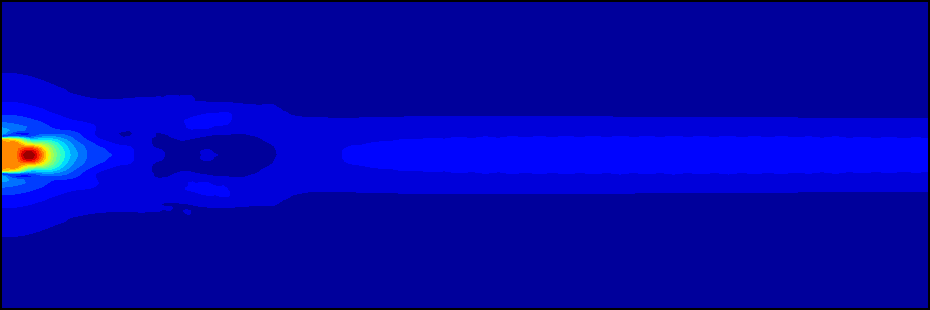
\includegraphics[width=0.48\linewidth]{figs/Re265-01} \hspace{0.1cm}
  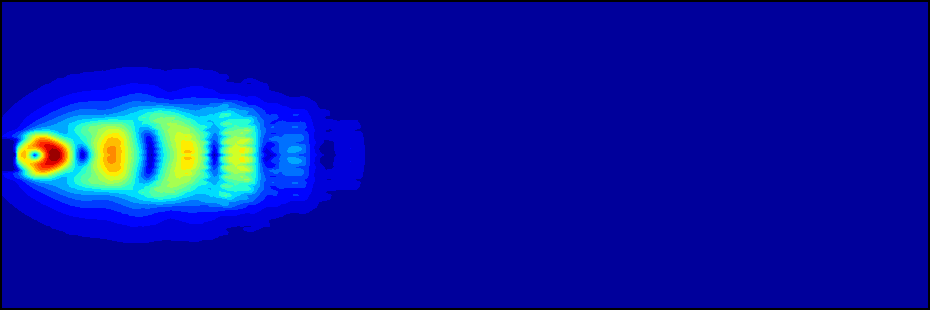
\includegraphics[width=0.48\linewidth]{figs/Re265-02} \\[0.3cm]
  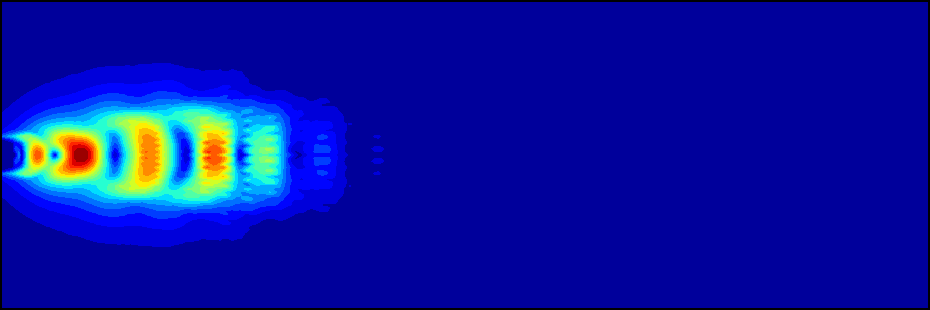
\includegraphics[width=0.48\linewidth]{figs/Re265-03} \hspace{0.1cm}
  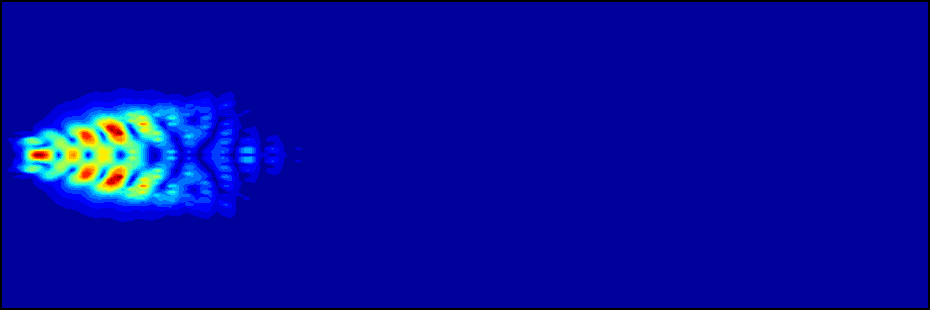
\includegraphics[width=0.48\linewidth]{figs/Re265-04}
  First modes for $\text{Re} = 265$.
\end{center}
\begin{center}
  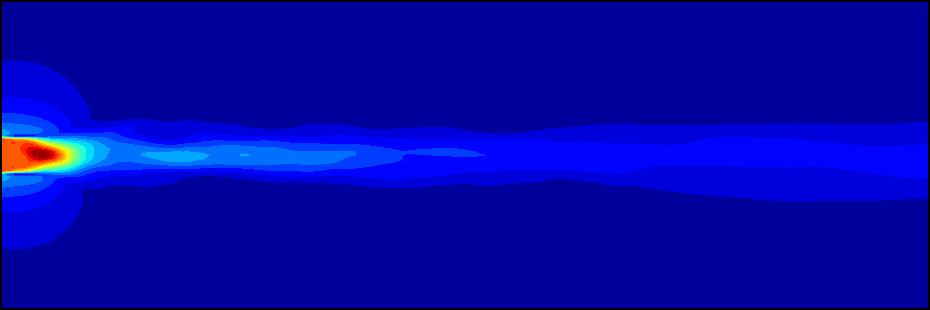
\includegraphics[width=0.48\linewidth]{figs/Re2580-01} \hspace{0.1cm}
  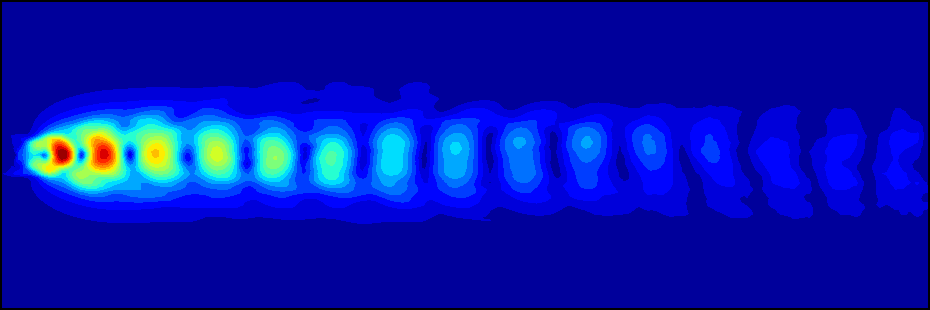
\includegraphics[width=0.48\linewidth]{figs/Re2580-02} \\[0.3cm]
  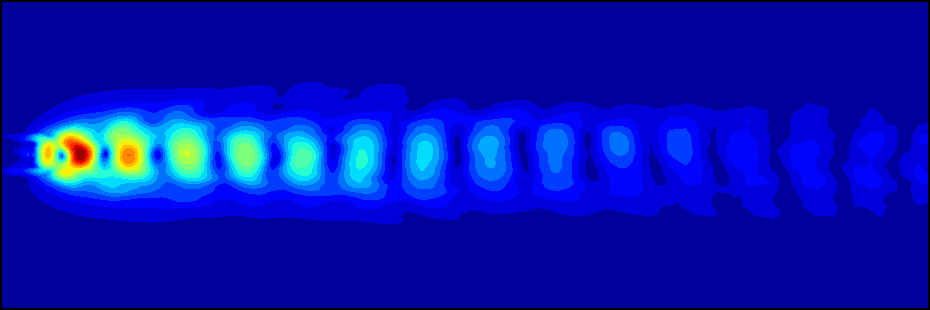
\includegraphics[width=0.48\linewidth]{figs/Re2580-03} \hspace{0.1cm}
  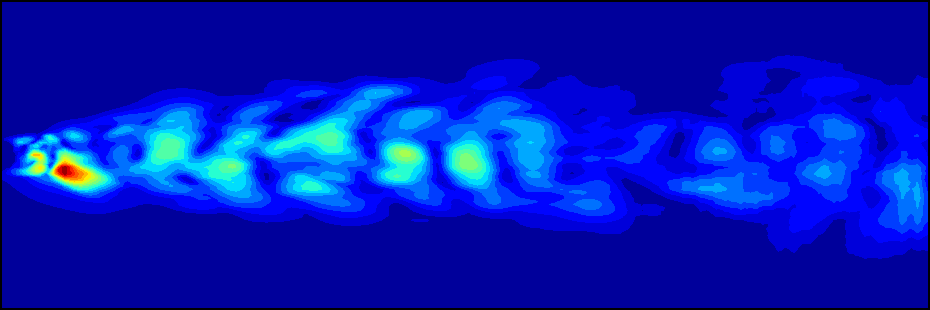
\includegraphics[width=0.48\linewidth]{figs/Re2580-04}
  First modes for $\text{Re} = 2580$.
\end{center}
\begin{center}
  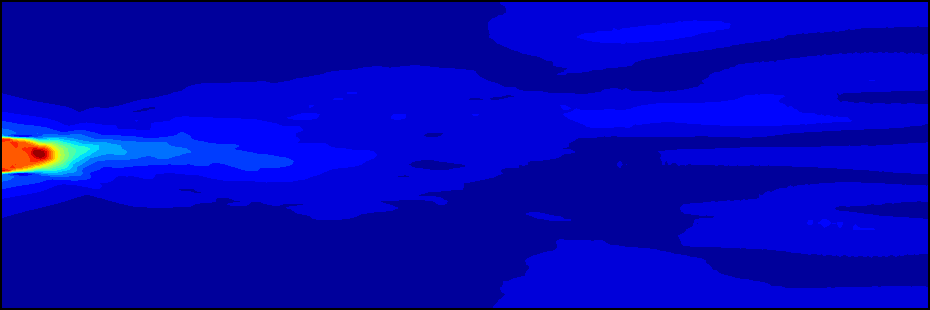
\includegraphics[width=0.48\linewidth]{figs/Re40000-01} \hspace{0.1cm}
  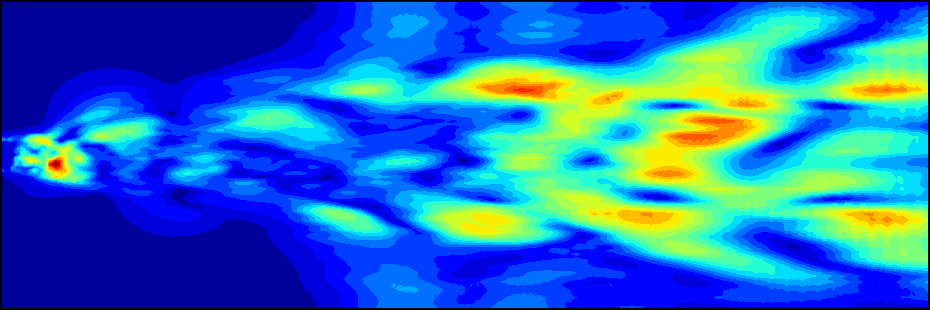
\includegraphics[width=0.48\linewidth]{figs/Re40000-02} \\[0.3cm]
  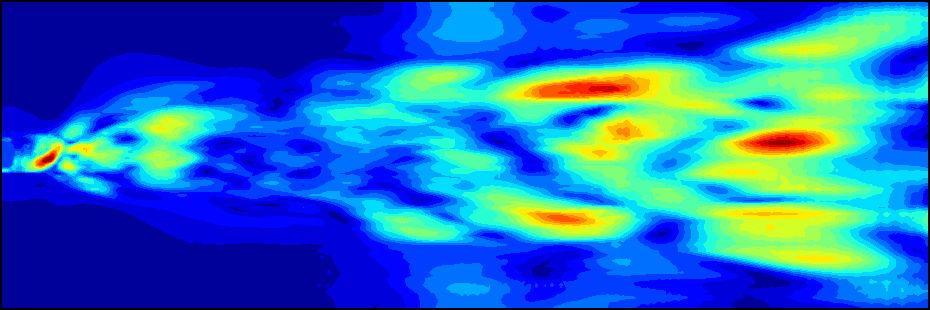
\includegraphics[width=0.48\linewidth]{figs/Re40000-03} \hspace{0.1cm}
  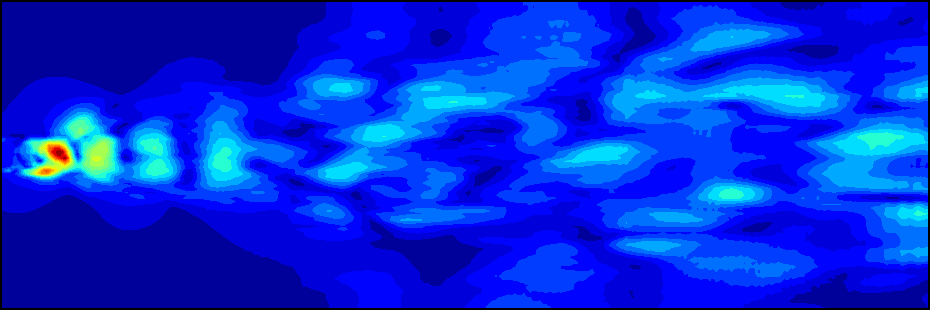
\includegraphics[width=0.48\linewidth]{figs/Re40000-04}
  First modes for $\text{Re} = 40000$.
\end{center}

\section*{\LARGE Discussion}

In all cases, about 30 modes suffice to cover $90\%$ of the energy content. For
low Reynold's number cases, the number of considerably smaller. For the other
cases, the energy decay is consistent, suggesting this decay rate may be
representative for a wider range of parameters. The first mode is always
``laminar'' and the following two modes appear to be phase-shifted principal
oscillations. Higher modes provide turbulent content.

For the kinds of flows considered here, POD appears an attractive method for
constructing the reduced bases required by ROMs.

\end{multicols}

\end{document}
